\chapter{MULTILAYER DRIPPING HANDRAIL}
\thispagestyle{empty}

Accretion disc model developed for the purpose of this study is constructed of $n$ times $m$ individual cells arranged in concentric circular grid, where $n$ is the number of concentric layers and $m$ number of cells in its layers. 

Each cell holds a set of parameters and its behavior is governed by set of oridinary differential equations derived from MSMM so fundamentally every cell is its own \emph{dripping faucet}. Layers move in the same direction\footnote{Direction is arbitrary and a matter of perspective (i.e. top vs. bottom view)} with keplerial orbital speeds relative to the outermost layer, which move by exacly one cell angular length in one simulation step. In every simulation step, there is a predefined constant mass influx into the outermost layer. This influx could come from specific azimuth or it could be distributed in some probabilistic manner from a wider range of angels.

As the simulation progresses the mass is distributed in tangential direction by the orbital movement of layers and in radial direction by overflow from individual cells. This radial mass transfer is unidirectional towards the grid center and is triggered by reaching a critical condition of MSMM in specific cells. 

Cell parameters and radial mass overflow are logged separately and later used to compute the radiative output, which is strongly dependent on radial mass transfer through changes in cell temperature and energy losses in gravitational potential of the imagined central body. 

Based on its characteristics, this model is called a \emph{Multilayer Dripping Handrail} and hereinafter, it shall be referenced as MDH.

\section{MDH grid structure}

The cells are arranged in concentric circual grid of $n$ layers and $m$ cells in each layer. Layers are denoted by $i \in [0, n-1]$, with the outremost layer having the index $i = 0$. Individual cells in each layer are denoted by $j \in [0, m-1]$\footnote{Direction of $j$ index iteration is arbitrary and depends on inplementation}. Figure \ref{fig:grid_states} shows simplified representation of this concentric simulation grid in its initial state. 

\begin{figure}
\centering
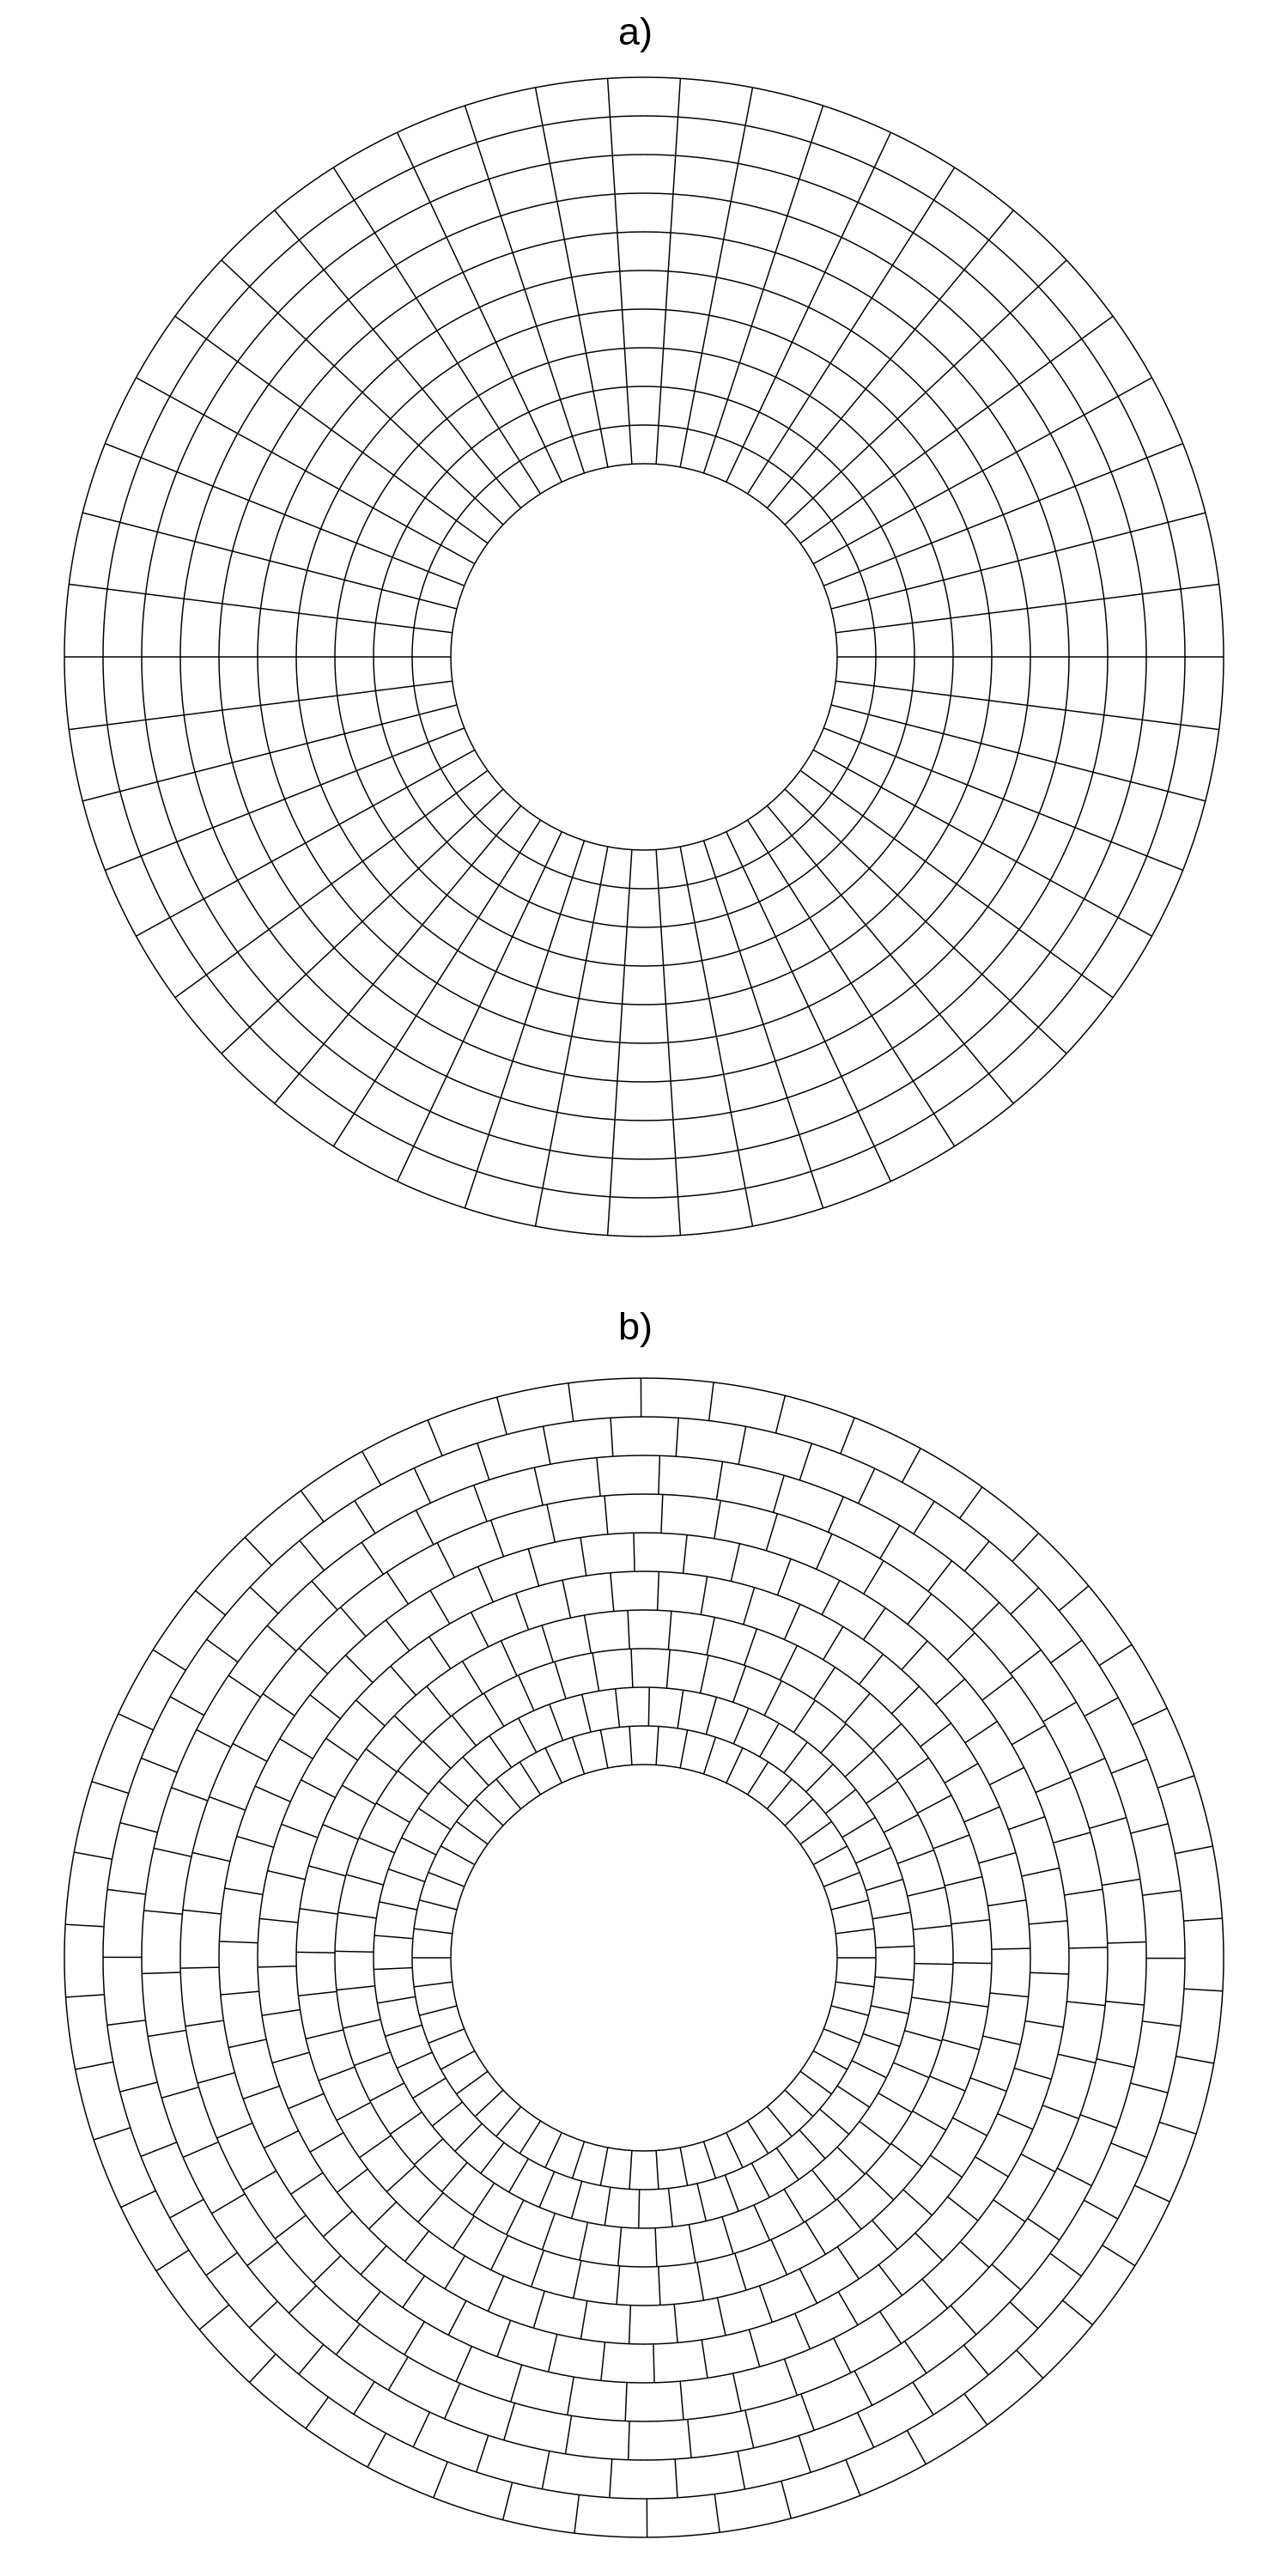
\includegraphics[width=0.75\columnwidth]{img/grid_states.png}
\caption{Simulation grid states: a) Initial unshifted state b) Shifted state after arbitrary number of simulation steps}
\label{fig:grid_states}
\end{figure}

Whole simultaion grid acts like cellular automaton (CA). Cellular automata models usualy implement some kind of simple condition or set of conditions (e.g. Conway's game of life, see \cite{gardner1970}), to decide simulation development for the next step. In the case of model created by \cite{yonehara1997}, there is a simple mass limit condition triggering the radial mass trasfer. MDH takes this concept further and implements the condition as critical value of \emph{spring elongation} $z$ of MSMM, which is the solution of its ODE system solved repeatedly in every step. 

\section{Cell definition}
Individual cells are defined by a set of parameters, that are necessary for runing the  MDH model. These parameters are listest in table \ref{table:mdh_cell_parameters} and following sections discuss some of them in detail.

\vspace{5mm}

\begin{table}[h]
\begin{center}
\begin{tabular}{r|l}
$i$			& Layer index \\
$j$			& Cell index \\
$r$			& Orbital radius \\
$\theta$		& Orbital azimuth \\ 
$g$			& Gravitational acceleration relative to outermost layer \\
$z$			& MSMM \emph{spring elongation}  \\
$v$			& MSMM \emph{velocity} \\
$m$			& Mass contained by cell \\
$\Delta m$ 	& Mass change since previous step \\
$\gamma$		& Constant MSMM dumpening parameter \\
$k$			& MSMM \emph{spring stiffness} \\
$T$			& Cell temperature
\end{tabular}
\caption{MDH cell parameters}
\label{table:mdh_cell_parameters}
\end{center}
\end{table}

\subsection{MDH model geometry}
Position and size of specific cell in MDH model, arise from \emph{real world} geometry of modeled accreation disc system. Parameters in question, are the orbital radius $r$ and orbital azimuth $\theta$. To define the oribital radius $r$, first the inner $r_{in}$ and outer $r_out$ radii of the imagined accretion disc must be defined. The modeled system is considered to be a typical CV star, therefore in the first approximation $r_{in}$, that defines the boundary layer between accretion disc and central body, is set to be equal to the radius of the white dwarf and according to \cite{shapiro1983} $r_{in}$ is be obtained as:

\begin{equation}
    r_{in} \sim M_p^{-1/3},
\end{equation}

where $M_p$ represents mass of the primary component (i.e the white dwarf). Outer radius $r_{out}$ represents the outer edge of accretion disc, that is constrained by the Roche potential (citace!!!). Outer radius $r_{out}$ is then calculated as:

\begin{equation}
    r_{out} = d \cdot \frac{M_{s}}{3 \cdot (M_p+M_{s})^{1/3}},
\end{equation}

where $d$ represents the distance between binary system components and $M_s$ represents mass of the secondary donor star. Space between $r_{in}$ and $r_{out}$ is discretize into regulary spaced interval according to chosen radial dimension $n$:

\begin{equation} \label{eq:cell_radius}
    r_i = r_{in} + (n - i - 1) \cdot \frac{r_{out} - r_{in}}{n - 1},
\end{equation}

\subsection{Azimuth and angular velocity profile}
Accretion disc layers (i.e. rings) are divided into equaly spaced $m$ number of cells. Angular position is expresed by its orbital azimuth $\theta \in [0, 2\pi]$. Because orbits a considered to be \emph{Keplerian}, and for simplicity circular, layers move at differing angular velocities. MDH model defines, that the outermost layer moves by exacly one \emph{cell angular length} $d\theta$ in one simulation step, therefore the angular velocity at the outermost layer $i=0$ is:

\begin{equation}
f_{\omega(i=0)} \equiv 1.
\end{equation}

Angular velocity at arbitrary layer is defined as:

\begin{equation}
\omega_i = \frac{v_i}{r_i},
\end{equation}

where $v_i$ represents the orbital velocity and $r_i$ is result of equation \ref{eq:cell_radius}. The cell specific orbital velocity is obtained as:

\begin{equation}
v_i = \sqrt{\frac{G \cdot M_p}{r_i}}.
\end{equation}

A



\subsection{Gravity profile}

\subsection{MSMM parameters}





\subsection{Temperature profile}


MSMM ODE system ... 

\begin{equation}
    \D{}{t} \left(m \D{z}{t}\right) = -kz - \gamma\D{z}{t} + mg,
\end{equation}
\begin{equation}
    \D{m}{t} = Q = const.,
\end{equation}

MSMM \emph{spring stiffness} ...

\begin{equation}
    \begin{aligned}
        & k~= 
        \begin{cases}
            -11{,}4m + 52{,}5 \hspace{10mm} (m < 4{,}61) \\
            \hspace{10mm} 0 \hspace{21mm} (m \ge 4{,}61 ),
        \end{cases}
    \end{aligned}
\end{equation}

Mass redistribution criteria ...

\begin{equation}
    m_r = 0.2m+0.3.
\end{equation}



Layer orbital period ...

\begin{equation}
    T_{i=0} = \sqrt{\frac{4 \pi^2 r_{out}^3}{G M_{p}}}.
\end{equation}

Timestep size ...

\begin{equation}
    h = T_{i=0} / m,
\end{equation}

Layer radius ...



